\begin{figure}[htp]
	\centering
	\subfloat[\(\mesh{\phi_{3}}\)]
	{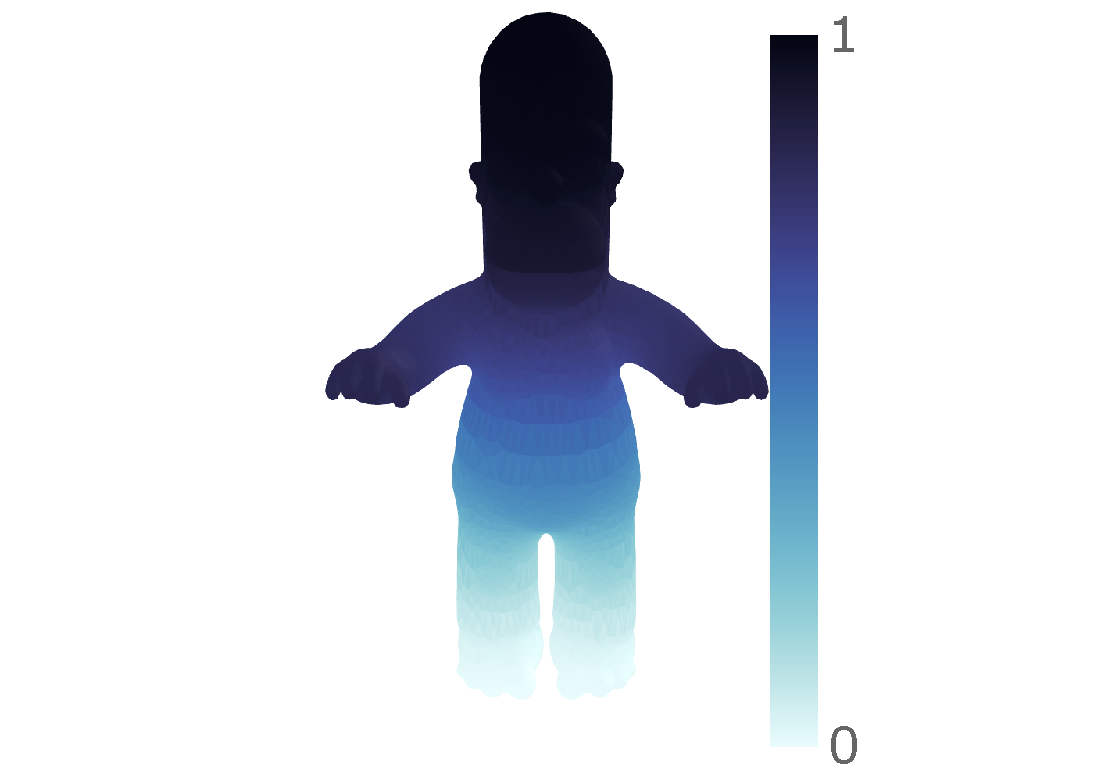
\includegraphics[trim={156 8 21 6},clip,width=.25\textwidth]{homer_rank2_lam1-325328e-03_norm.pdf}} % chktex 8
	\hfill
	\subfloat[\(\mesh{\phi_{4}}\)]
	{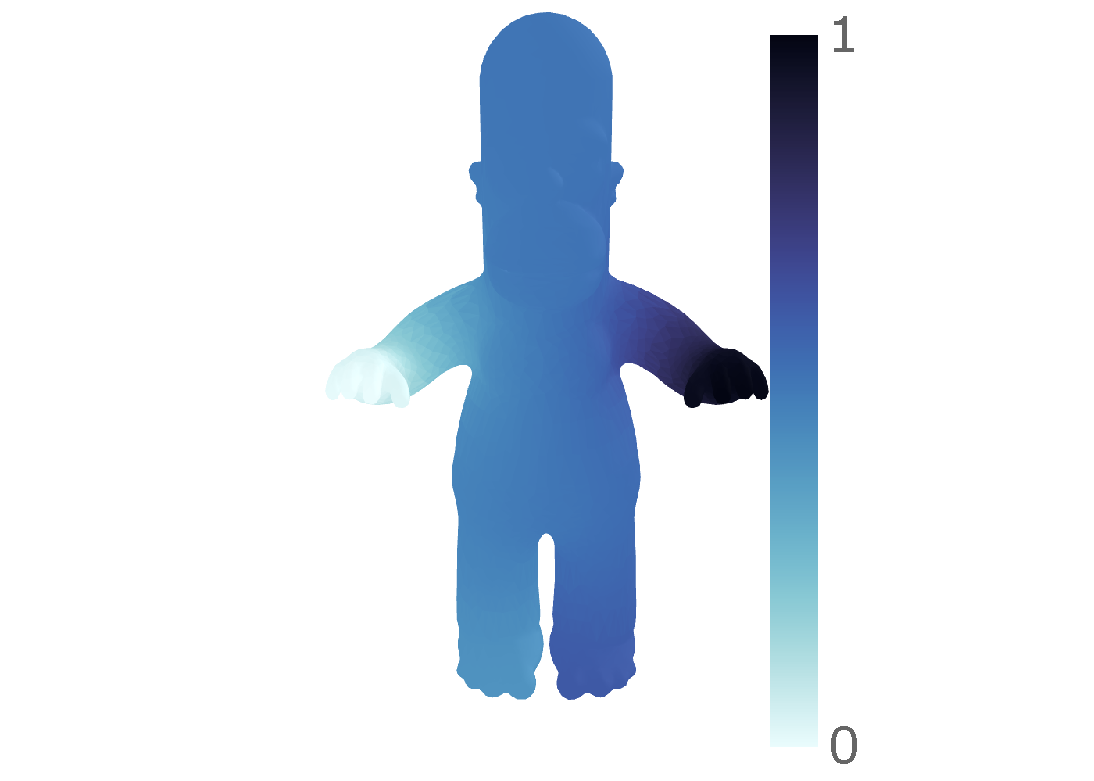
\includegraphics[trim={156 8 21 6},clip,width=.25\textwidth]{homer_rank3_lam2-425344e-03_norm.pdf}} % chktex 8
	\hfill
	\subfloat[\(\mesh{\phi_{5}}\)]
	{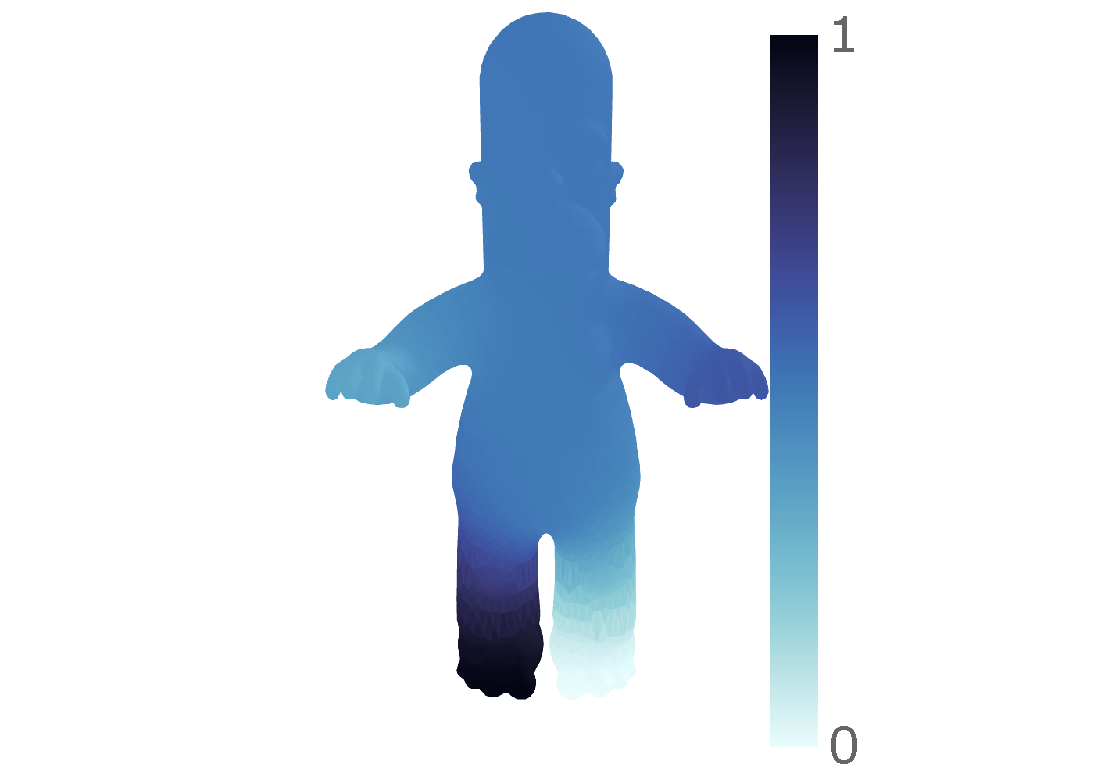
\includegraphics[trim={156 8 21 6},clip,width=.25\textwidth]{homer_rank4_lam2-706937e-03_norm.pdf}} % chktex 8
	\hfill
	\subfloat[\(\mesh{\phi_{6}}\)]
	{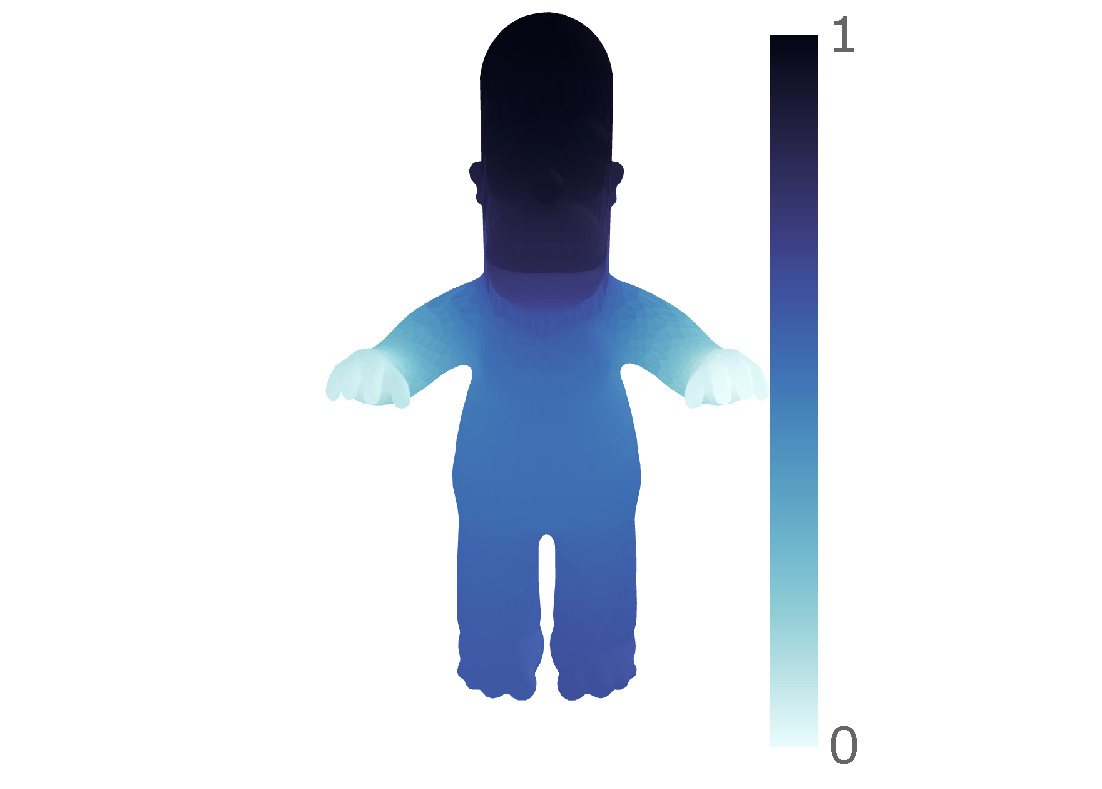
\includegraphics[trim={156 8 21 6},clip,width=.25\textwidth]{homer_rank5_lam2-851096e-03_norm.pdf}} % chktex 8
	\newline
	\subfloat[\(\mesh{\phi_{7}}\)]
	{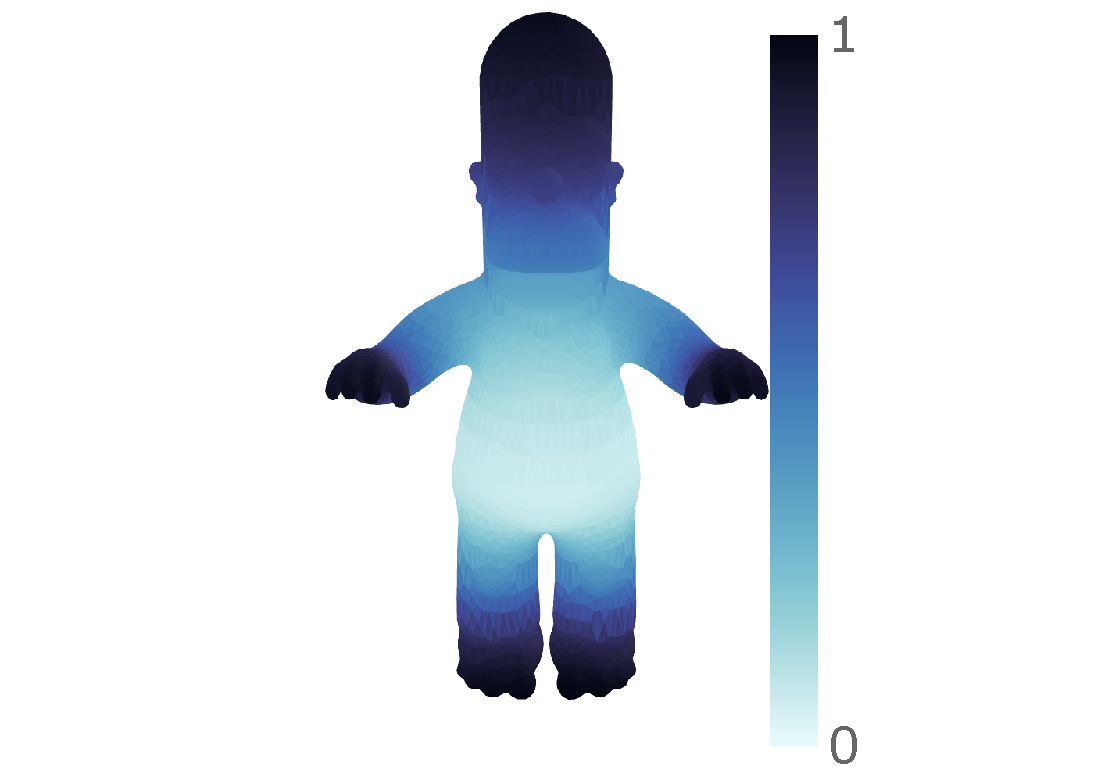
\includegraphics[trim={156 8 21 6},clip,width=.25\textwidth]{homer_rank6_lam7-806422e-03_norm.pdf}} % chktex 8
	\hfill
	\subfloat[\(\mesh{\phi_{8}}\)]
	{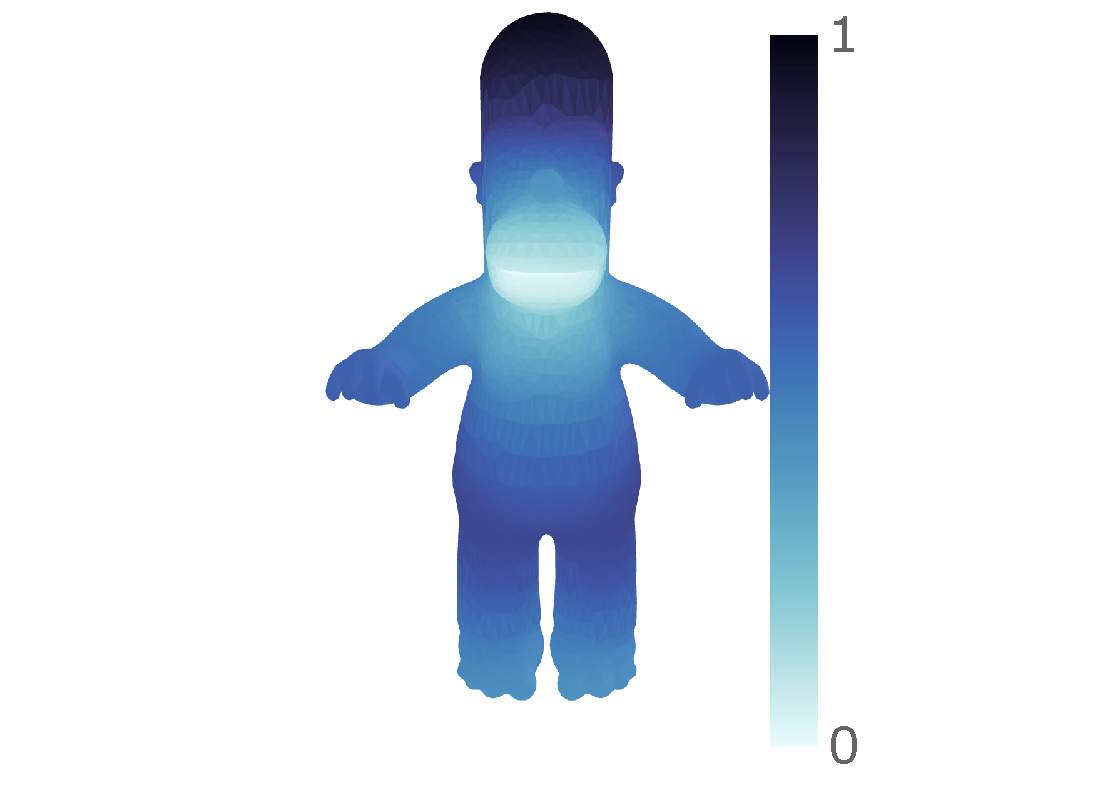
\includegraphics[trim={156 8 21 6},clip,width=.25\textwidth]{homer_rank7_lam1-164387e-02_norm.pdf}} % chktex 8
	\subfloat[\(\mesh{\phi_{9}}\)]
	{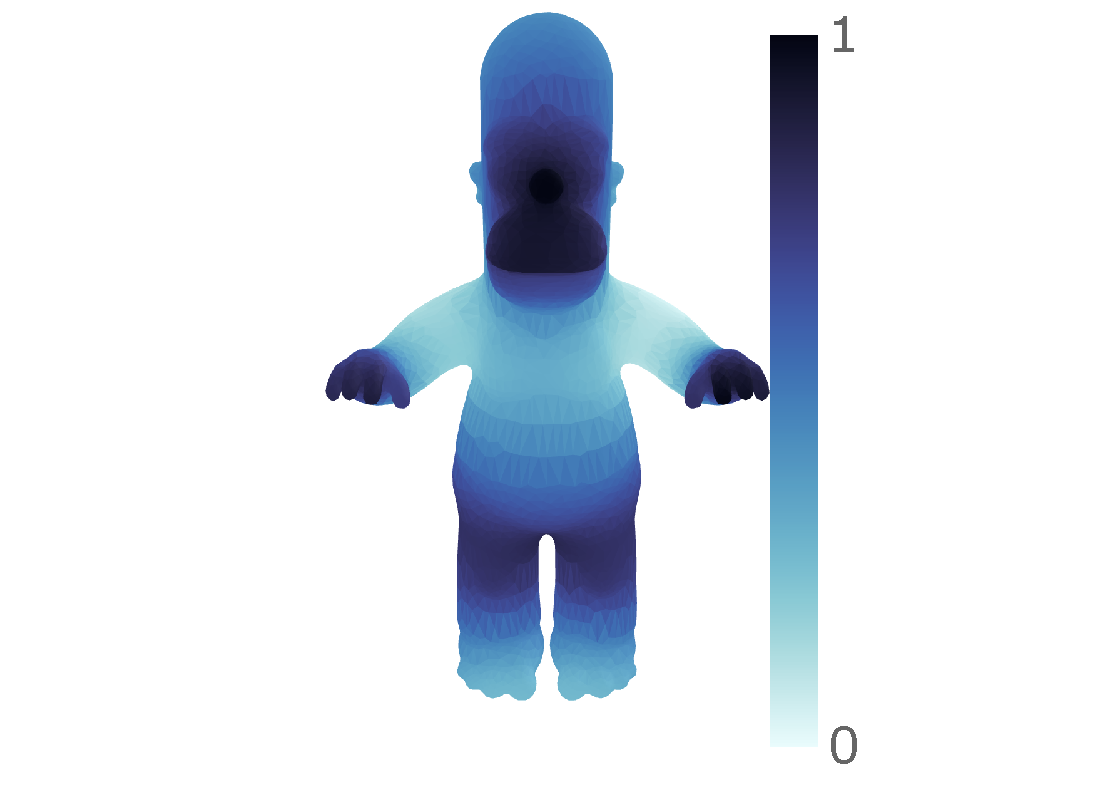
\includegraphics[trim={156 8 21 6},clip,width=.25\textwidth]{homer_rank8_lam1-738974e-02_norm.pdf}} % chktex 8
	\hfill
	\subfloat[\(\mesh{\phi_{10}}\)]
	{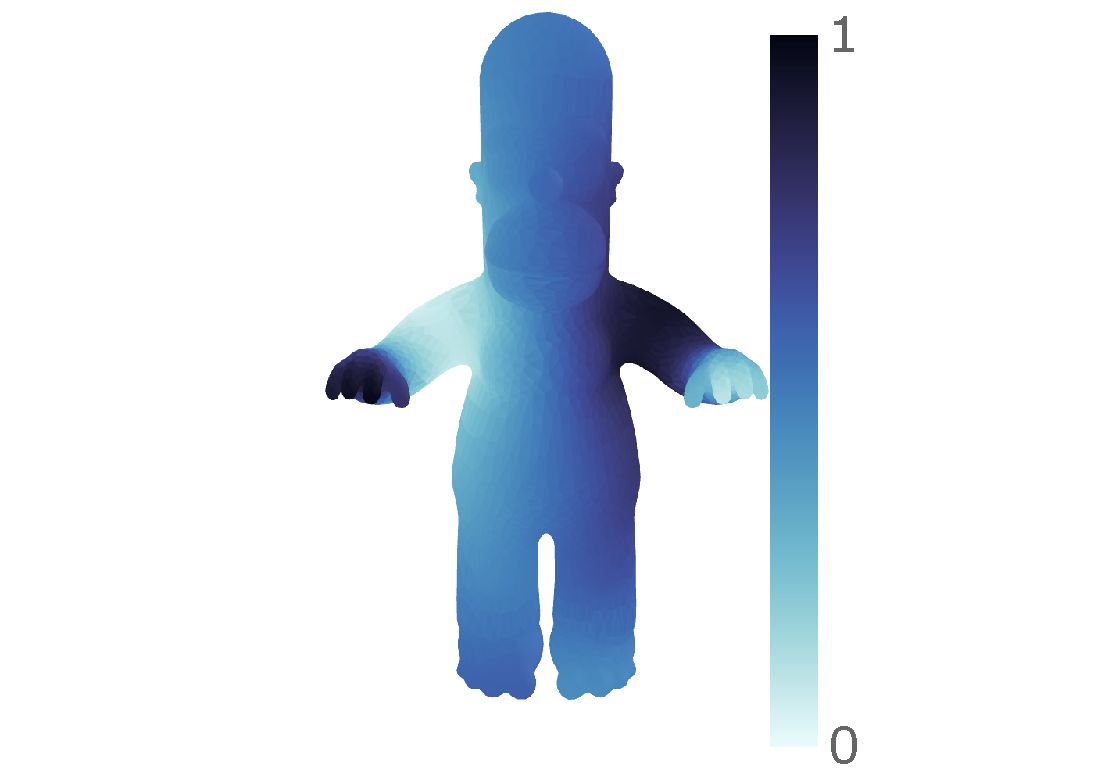
\includegraphics[trim={156 8 21 6},clip,width=.25\textwidth]{homer_rank9_lam1-827015e-02_norm.pdf}} % chktex 8
	\caption[
		Some eigenvectors of the mesh Laplacian of an example mesh
	]{
		The third to tenth eigenvectors of the mesh Laplacian of a Homer Simpson mesh ordered by increasing eigenvalue (frequency).
		In total \(\imax=\num{1275}\) basis functions of the \(\num{5103}\) vertex mesh were computed.
		Whilst the eigenvectors are defined on the vertices, the values have been averaged onto the faces for the plot.
	}\label{fig:chapter4_eigenhomers}
\end{figure}
